162. \begin{figure}[ht!]
\center{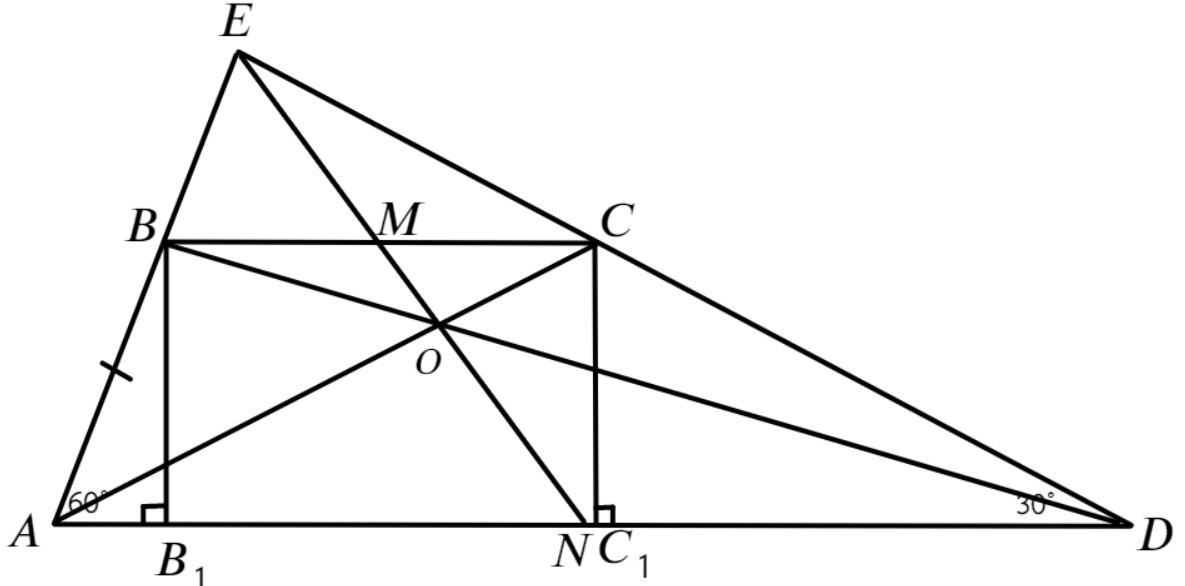
\includegraphics[scale=0.35]{g8-162.png}}
\end{figure}\\
а) Опустим высоты $BB_1$ и $CC_1.$ Тогда $BB_1=AB\ \sin(60^\circ)=2\cdot \cfrac{\sqrt{3}}{2}=\sqrt{3},\ CD=CC_1:\sin(60^\circ)=\sqrt{3}:\cfrac{1}{2}=2\sqrt{3}.$\\
б) $AB_1=AB\ \cos(60^\circ)=2 \cdot \cfrac{1}{2}=1,\ B_1C_1=BC=2,\ C_1D=CD\ \cos(30^\circ)=2\sqrt{3}\cdot \cfrac{\sqrt{3}}{2}=3.$ Тогда $S_{ABCD}=\sqrt{3}\cdot\cfrac{2+1+2+3}{2}=4\sqrt{3}.$\\
в) Треугольники $AOD$ и $BOC$ подобны по двум углам (вертикальные и накрест лежащие), значит их высоты, опущенные из точки $O,$ относятся, как и стороны, с коэффициентом $\cfrac{AD}{BC}=\cfrac{6}{2}=3.$ Сумма их высот равна высоте трапеции, значит высота треугольника $AOD$ равна $\cfrac{3}{4}\sqrt{3},$ а его площадь $S_{\Delta AOD}=\cfrac{1}{2}\cdot\cfrac{3}{4}\sqrt{3}\cdot6=\cfrac{9\sqrt{3}}{4}.$\\
г) Продлим боковые стороны трапеции до пересечения, тогда точка их пересечения лежит на одной прямой с серединами оснований (и с точкой пересечения диагоналей, но в нашей задаче это не требуется). Тогда $\angle AED=180^\circ-30^\circ-60^\circ=90^\circ.$ Отрезки $EN$ и $EM$ являются медианами, проведёнными из прямого угла, значит $MN=EN-EM=\cfrac{1}{2}AD-\cfrac{1}{2}BC=\cfrac{1}{2}(AD-BC)=\cfrac{1}{2}\cdot4=2$.\\
